%%%%%%%%%%%%%%%%%%%%%%%%%%%%%%%%%%%%%%%%%%%%%%%%%%%%%%%%%%%
% --------------------------------------------------------
%  _____           
% |_   _|_ _ _   _ 
%   | |/ _` | | | |
%   | | (_| | |_| |
%   |_|\__,_|\__,_|
%
% LaTeX2e Template
% Version 2.6.0 (21/04/2026)
%
% Author: 
% Guillermo Jimenez (memo.notess1@gmail.com)
% 
% License:
% Creative Commons CC BY 4.0
% --------------------------------------------------------
%%%%%%%%%%%%%%%%%%%%%%%%%%%%%%%%%%%%%%%%%%%%%%%%%%%%%%%%%%%
% --------------------------------------------------------
% Github Repository:
% https://github.com/MemoJimenez/Tau-class
% --------------------------------------------------------
%%%%%%%%%%%%%%%%%%%%%%%%%%%%%%%%%%%%%%%%%%%%%%%%%%%%%%%%%%%

\documentclass[9pt,a4paper,twocolumn,twoside]{tau-class/tau}
\usepackage[english]{babel}

% Spanish babel recomendation
% \usepackage[spanish,es-nodecimaldot,es-noindentfirst]{babel} 

%----------------------------------------------------------
% Title & Authors/Affiliations
%----------------------------------------------------------

\doctype{Thesis Report}
\title{Spatial Tensor Simulation}

%----------------------------------------------------------

\author[a,1]{Alejandro Ouslan\thanks{\href{mailto:alejandro.ouslan@upr.edu}{alejandro.ouslan@upr.edu} (A. One)}}

%----------------------------------------------------------

\affil[a]{University of Puerto Rico, Mayaguez}

%----------------------------------------------------------
% Document-, Footer- information
%----------------------------------------------------------

\dates{This manuscript was compiled on \today}

\docinfo{}

%----------------------------------------------------------

\footinfo{st\_repl (v.1.1.0)}
\theday{\today}
\organization{Thesis Report}
\leadauthor{A. One et al.}

%----------------------------------------------------------
% Abstract and Keywords
%----------------------------------------------------------

\begin{abstract}    
  TBD
\end{abstract}

%----------------------------------------------------------

\keywords{TBD}

%----------------------------------------------------------

\begin{document}
		
    \maketitle 
    \thispagestyle{firststyle}
    
%----------------------------------------------------------



\section{Spatial Data}

    \taustart{S}patial data can be easily generated using a simple 
    grid. For the purposes of comparing how spatial smoothers 
    behaves we will ganarte a small squire grid of $10 \times 10$.
    The following figure shows the grid used for this simulation. 

\begin{figure}[H]
	\centering
	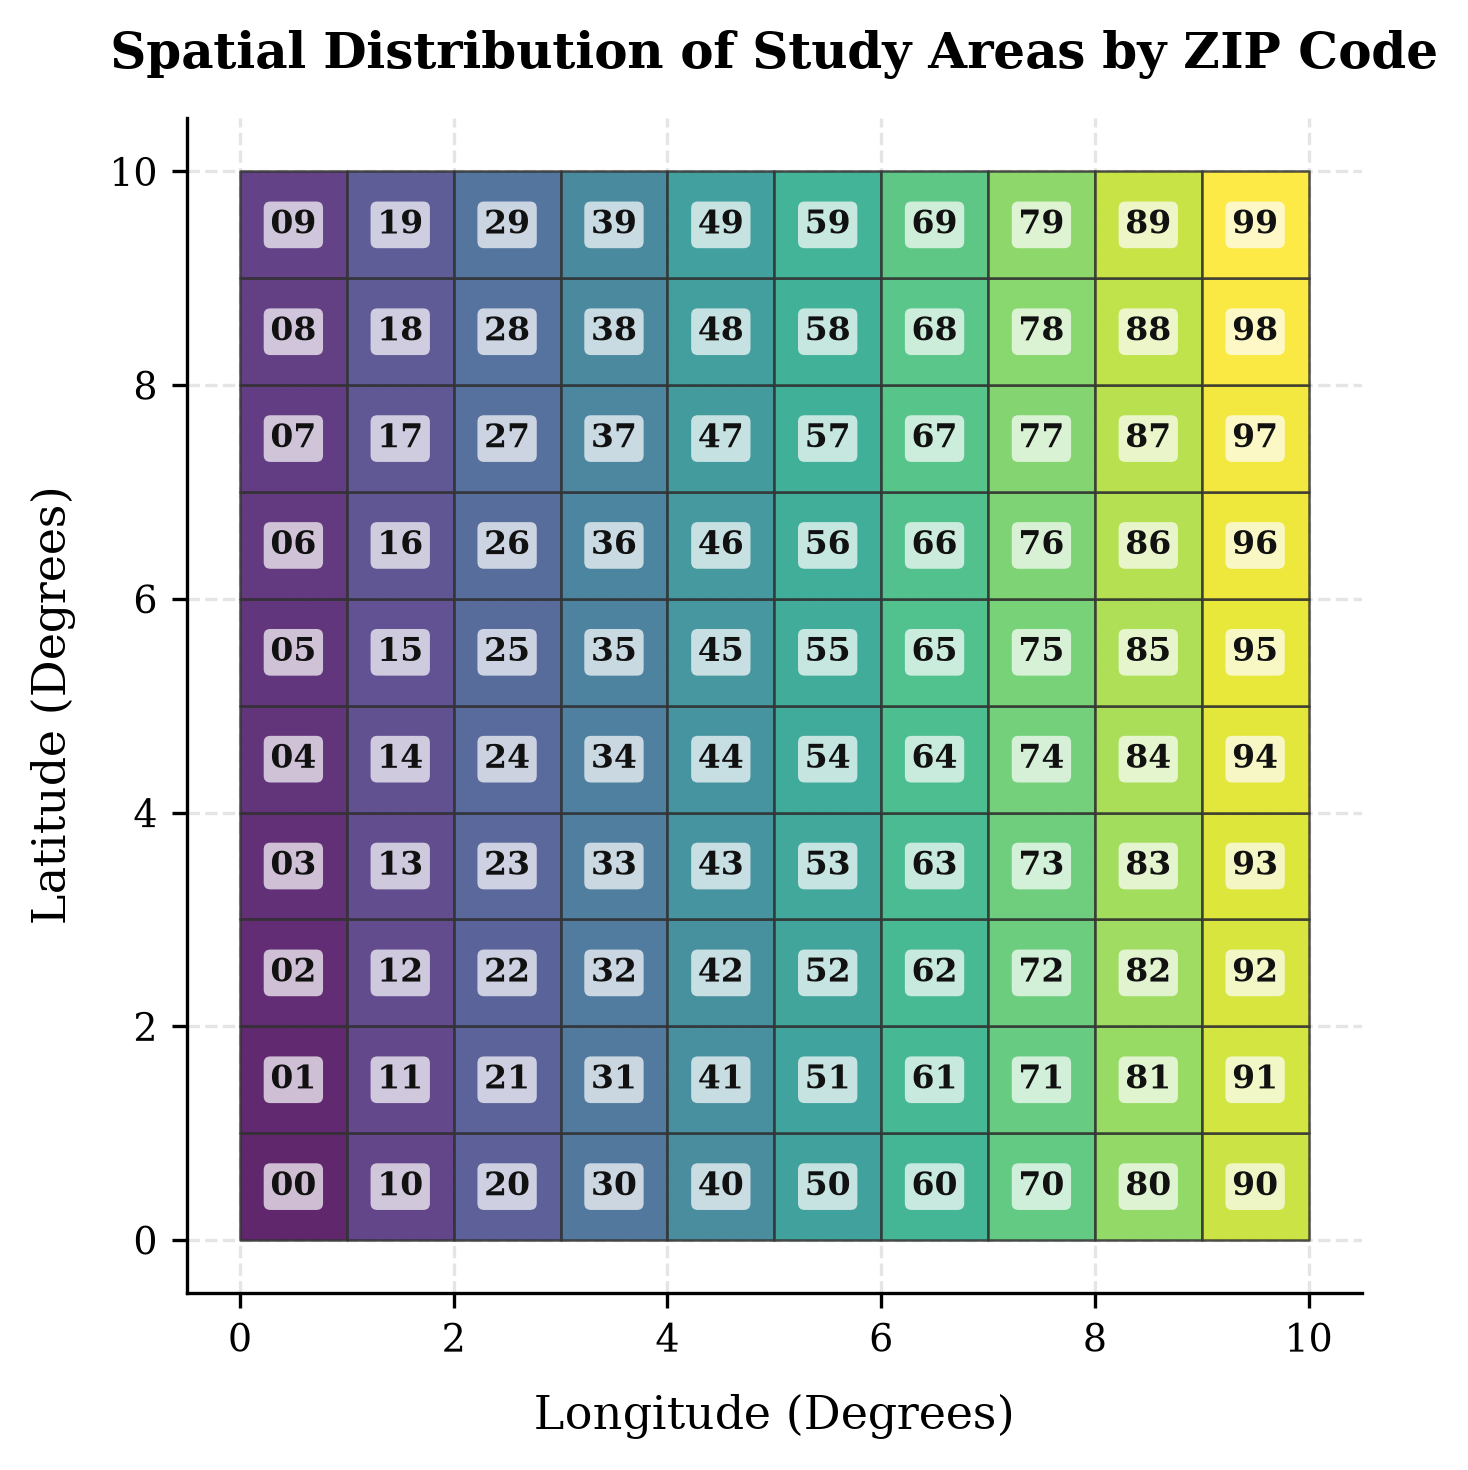
\includegraphics[width=0.4\textwidth]{figures/zip_grid_map.png}
  \label{zip_grid}
	\caption{Simulated Zipcode Grid Map}
\end{figure}


As this not a single point in time, we look how this each spatial agent 
behaves thought space. This this we will generate a balance panel dataset \cite{chamberlain1984panel}


This simulated will be generate an outcome variable that it distributse from a normal distributions 
were the data is infunced spatialy by its neoughrs. This can be summerized with the follwoign model 

\begin{equation}
  \begin{split}
    Y &\sim N(\alpha + \beta_1X_1 + \beta_2X_2 + \rho W Y) \\
    X_i &\sim N(2,3), \quad \text{ For } 1,2,3
  \end{split}
  \label{eq:simple_sar}
\end{equation}




%----------------------------------------------------------

\printbibliography

%----------------------------------------------------------

\end{document}
